% Phase 37 conference paper draft -- CONFIDENTIAL, private repository only.
% Target: Deployable AI Workshop at AAAI-27 (see VENUE.md), long paper, 7 pages + references/appendix,
% double-blind. Do not upload, post, share or submit until the authors lift the confidentiality rules.
%
% Build: put aaai2027.sty and aaai2027.bst from https://aaai.org/authorkit27/ next to this file, run
%   python scripts/paper_figures.py      (from the repository root; writes generated/*)
%   pdflatex paper && bibtex paper && pdflatex paper && pdflatex paper
% Every number in the text is a macro from generated/numbers.tex (trace: generated/NUMBERS_TRACE.md).

\def\year{2027}\relax
\documentclass[letterpaper]{article}
\usepackage[submission]{aaai2027}  % VERIFY the option name in the AAAI-27 kit (anonymous submission mode)
\usepackage{times}
\usepackage{helvet}
\usepackage{courier}
\usepackage[hyphens]{url}
\usepackage{graphicx}
\urlstyle{rm}
\def\UrlFont{\rm}
\usepackage{natbib}
\usepackage{caption}
\frenchspacing
\setlength{\pdfpagewidth}{8.5in}
\setlength{\pdfpageheight}{11in}
\usepackage{amsmath}
\usepackage{amssymb}
\usepackage{booktabs}
\usepackage{pgfplots}
\pgfplotsset{compat=1.17}
\pdfinfo{
/TemplateVersion (2027.1)
}
\setcounter{secnumdepth}{1}

% Generated by scripts/paper_figures.py from frozen files. Do not edit by hand.
\newcommand{\nGraphNodes}{\ensuremath{622}} % data/geospatial_v3/fort_kochi_osm_drive_v1_manifest.json /node_count
\newcommand{\nGraphEdges}{\ensuremath{1{,}358}} % data/geospatial_v3/fort_kochi_osm_drive_v1_manifest.json /edge_count
\newcommand{\nZones}{\ensuremath{4}} % data/geospatial_v3/fort_kochi_osm_drive_v1.json len(/zone_node_map)
\newcommand{\nShelters}{\ensuremath{5}} % data/geospatial_v3/fort_kochi_osm_drive_v1.json len(/shelter_node_map)
\newcommand{\nAmax}{\ensuremath{21}} % data/geospatial_v3/fort_kochi_osm_drive_v1.json zones x shelters + 1 (HOLD) = A_MAX
\newcommand{\nInitPop}{\ensuremath{312.1}} % data/eval_results/phase27/runs/A_{medium,high}.jsonl mean initial_population over primary-regime episodes (keyed by seed)
\newcommand{\nSeedsPerRegime}{\ensuremath{60}} % data/eval_results/phase27/analysis.json /budget/seeds_per_regime
\newcommand{\nEpisodesTotal}{\ensuremath{1{,}260}} % data/eval_results/phase27/analysis.json sum of /episodes/systems/*/*/episodes
\newcommand{\nBudgetHours}{\ensuremath{30.6}} % data/eval_results/phase27/analysis.json /budget/projection_full_hours_on_16_workers
\newcommand{\nPEpisodeSeconds}{\ensuremath{2{,}251}} % data/eval_results/phase27/analysis.json /budget/mean_episode_seconds/P
\newcommand{\nEOneDiff}{\ensuremath{-0.230}} % data/eval_results/phase27/analysis.json /bars/bar1/numbers/E1/mean_diff
\newcommand{\nEOneLo}{\ensuremath{-0.264}} % data/eval_results/phase27/analysis.json /bars/bar1/numbers/E1/ci95/0
\newcommand{\nEOneHi}{\ensuremath{-0.197}} % data/eval_results/phase27/analysis.json /bars/bar1/numbers/E1/ci95/1
\newcommand{\nEOnePairs}{\ensuremath{120}} % data/eval_results/phase27/analysis.json /bars/bar1/numbers/E1/n_pairs
\newcommand{\nRateA}{\ensuremath{23.7\,\%}} % data/eval_results/phase27/analysis.json /bars/bar1/numbers/E1/mean_rate_baseline
\newcommand{\nRateP}{\ensuremath{0.7\,\%}} % data/eval_results/phase27/analysis.json mean_rate_baseline + mean_diff (/bars/bar1/numbers/E1)
\newcommand{\nRelReduction}{\ensuremath{97\,\%}} % data/eval_results/phase27/analysis.json /bars/bar1/numbers/E1/relative_reduction
\newcommand{\nR}{\ensuremath{0.214}} % data/eval_results/phase27/analysis.json /bars/bar1/numbers/R_P_over_A2
\newcommand{\nRpct}{\ensuremath{21.4\,\%}} % data/eval_results/phase27/analysis.json /bars/bar1/numbers/R_P_over_A2
\newcommand{\nQtwoCandidates}{\ensuremath{4{,}798}} % data/eval_results/phase27/analysis.json /bars/bar2/numbers/candidates
\newcommand{\nQtwoBorderline}{\ensuremath{227}} % data/eval_results/phase27/analysis.json /bars/bar2/numbers/borderline_excluded
\newcommand{\nQtwoGraded}{\ensuremath{4{,}571}} % data/eval_results/phase27/analysis.json /bars/bar2/numbers/graded
\newcommand{\nFBJoint}{\ensuremath{179}} % data/eval_results/phase27/analysis.json /bars/bar2/numbers/false_blocks/joint
\newcommand{\nFBProduct}{\ensuremath{243}} % data/eval_results/phase27/analysis.json /bars/bar2/numbers/false_blocks/product_of_marginals
\newcommand{\nFBSeparate}{\ensuremath{243}} % data/eval_results/phase27/analysis.json /bars/bar2/numbers/false_blocks/separate_checks
\newcommand{\nFAJoint}{\ensuremath{0}} % data/eval_results/phase27/analysis.json /bars/bar2/numbers/false_accepts/joint
\newcommand{\nFAProduct}{\ensuremath{0}} % data/eval_results/phase27/analysis.json /bars/bar2/numbers/false_accepts/product_of_marginals
\newcommand{\nFASeparate}{\ensuremath{0}} % data/eval_results/phase27/analysis.json /bars/bar2/numbers/false_accepts/separate_checks
\newcommand{\nMcNJointOnly}{\ensuremath{64}} % data/eval_results/phase27/analysis.json /bars/bar2/numbers/mcnemar/product_of_marginals/joint_only_right
\newcommand{\nMcNOtherOnly}{\ensuremath{0}} % data/eval_results/phase27/analysis.json /bars/bar2/numbers/mcnemar/product_of_marginals/other_only_right
\newcommand{\nMcNSepJointOnly}{\ensuremath{64}} % data/eval_results/phase27/analysis.json /bars/bar2/numbers/mcnemar/separate_checks/joint_only_right
\newcommand{\nMcNSepOtherOnly}{\ensuremath{0}} % data/eval_results/phase27/analysis.json /bars/bar2/numbers/mcnemar/separate_checks/other_only_right
\newcommand{\nMcNp}{\ensuremath{1.08\times10^{-19}}} % data/eval_results/phase27/analysis.json /bars/bar2/numbers/mcnemar/product_of_marginals/p
\newcommand{\nFBReduction}{\ensuremath{26.3\,\%}} % data/eval_results/phase27/analysis.json /bars/bar2/numbers/false_block_reduction_vs_product
\newcommand{\nVarRatio}{\ensuremath{1.071}} % data/eval_results/phase27/analysis.json /bars/bar3/numbers/median_var_ratio
\newcommand{\nQthreeStates}{\ensuremath{50}} % data/eval_results/phase27/analysis.json /bars/bar3/numbers/states
\newcommand{\nQfourStates}{\ensuremath{400}} % data/eval_results/phase27/analysis.json /bars/bar4/numbers/states
\newcommand{\nQfourFA}{\ensuremath{0}} % data/eval_results/phase27/analysis.json /bars/bar4/numbers/states_with_false_accept
\newcommand{\nQfourUpper}{\ensuremath{0.0075}} % data/eval_results/phase27/analysis.json /bars/bar4/numbers/cp95_upper
\newcommand{\nGroupsHold}{\ensuremath{0.0}} % data/eval_results/phase27/analysis.json sum dispatched_groups / sum episodes, /episodes/systems/HOLD/{medium,high}
\newcommand{\nSafeHold}{\ensuremath{0.0}} % data/eval_results/phase27/analysis.json mean of /episodes/systems/HOLD/{medium,high}/mean_safe_arrivals
\newcommand{\nFailHold}{\ensuremath{0.0\,\%}} % data/eval_results/phase27/analysis.json mean of /episodes/systems/HOLD/{medium,high}/mean_group_failure_rate
\newcommand{\nGroupsA}{\ensuremath{16.6}} % data/eval_results/phase27/analysis.json sum dispatched_groups / sum episodes, /episodes/systems/A/{medium,high}
\newcommand{\nSafeA}{\ensuremath{228.1}} % data/eval_results/phase27/analysis.json mean of /episodes/systems/A/{medium,high}/mean_safe_arrivals
\newcommand{\nFailA}{\ensuremath{23.7\,\%}} % data/eval_results/phase27/analysis.json mean of /episodes/systems/A/{medium,high}/mean_group_failure_rate
\newcommand{\nGroupsAtwo}{\ensuremath{16.6}} % data/eval_results/phase27/analysis.json sum dispatched_groups / sum episodes, /episodes/systems/A2/{medium,high}
\newcommand{\nSafeAtwo}{\ensuremath{223.8}} % data/eval_results/phase27/analysis.json mean of /episodes/systems/A2/{medium,high}/mean_safe_arrivals
\newcommand{\nFailAtwo}{\ensuremath{26.0\,\%}} % data/eval_results/phase27/analysis.json mean of /episodes/systems/A2/{medium,high}/mean_group_failure_rate
\newcommand{\nGroupsB}{\ensuremath{8.2}} % data/eval_results/phase27/analysis.json sum dispatched_groups / sum episodes, /episodes/systems/B/{medium,high}
\newcommand{\nSafeB}{\ensuremath{132.9}} % data/eval_results/phase27/analysis.json mean of /episodes/systems/B/{medium,high}/mean_safe_arrivals
\newcommand{\nFailB}{\ensuremath{4.1\,\%}} % data/eval_results/phase27/analysis.json mean of /episodes/systems/B/{medium,high}/mean_group_failure_rate
\newcommand{\nGroupsP}{\ensuremath{3.3}} % data/eval_results/phase27/analysis.json sum dispatched_groups / sum episodes, /episodes/systems/P/{medium,high}
\newcommand{\nSafeP}{\ensuremath{47.9}} % data/eval_results/phase27/analysis.json mean of /episodes/systems/P/{medium,high}/mean_safe_arrivals
\newcommand{\nFailP}{\ensuremath{0.7\,\%}} % data/eval_results/phase27/analysis.json mean of /episodes/systems/P/{medium,high}/mean_group_failure_rate
\newcommand{\nGroupsPnoFC}{\ensuremath{6.6}} % data/eval_results/phase27/analysis.json sum dispatched_groups / sum episodes, /episodes/systems/P-noFC/{medium,high}
\newcommand{\nSafePnoFC}{\ensuremath{104.4}} % data/eval_results/phase27/analysis.json mean of /episodes/systems/P-noFC/{medium,high}/mean_safe_arrivals
\newcommand{\nFailPnoFC}{\ensuremath{3.3\,\%}} % data/eval_results/phase27/analysis.json mean of /episodes/systems/P-noFC/{medium,high}/mean_group_failure_rate
\newcommand{\nGroupsPnoHyst}{\ensuremath{3.3}} % data/eval_results/phase27/analysis.json sum dispatched_groups / sum episodes, /episodes/systems/P-noHyst/{medium,high}
\newcommand{\nSafePnoHyst}{\ensuremath{47.9}} % data/eval_results/phase27/analysis.json mean of /episodes/systems/P-noHyst/{medium,high}/mean_safe_arrivals
\newcommand{\nFailPnoHyst}{\ensuremath{0.7\,\%}} % data/eval_results/phase27/analysis.json mean of /episodes/systems/P-noHyst/{medium,high}/mean_group_failure_rate
\newcommand{\nMigrationsP}{\ensuremath{2}} % data/eval_results/phase27/analysis.json sum of /episodes/systems/P/{medium,high}/migrations
\newcommand{\nArrErrP}{\ensuremath{0}} % data/eval_results/phase27/analysis.json max over {medium,high} of /episodes/systems/P/<regime>/median_arrival_abs_error_steps
\newcommand{\nPvBDiff}{\ensuremath{-0.034}} % data/eval_results/phase27/analysis.json /secondary/P_vs_B/mean_diff
\newcommand{\nPvBLo}{\ensuremath{-0.049}} % data/eval_results/phase27/analysis.json /secondary/P_vs_B/ci95/0
\newcommand{\nPvBHi}{\ensuremath{-0.019}} % data/eval_results/phase27/analysis.json /secondary/P_vs_B/ci95/1
\newcommand{\nLatCertPfifty}{\ensuremath{288}} % data/eval_results/phase27/latency.json /0/certify_only_ms/p50
\newcommand{\nLatCertPninetyfive}{\ensuremath{1{,}059}} % data/eval_results/phase27/latency.json /0/certify_only_ms/p95
\newcommand{\nLatEtePfifty}{\ensuremath{6.6}} % data/eval_results/phase27/latency.json /0/end_to_end_ms/p50 / 1000
\newcommand{\nLatEtePninetyfive}{\ensuremath{13.9}} % data/eval_results/phase27/latency.json /0/end_to_end_ms/p95 / 1000
\newcommand{\nLatTargetCert}{\ensuremath{100}} % data/eval_results/phase27/latency.json /0/targets_ms/certify_only_p95
\newcommand{\nLatTargetEte}{\ensuremath{10}} % data/eval_results/phase27/latency.json /0/targets_ms/end_to_end_p95 / 1000
\newcommand{\nCovPNinety}{\ensuremath{0.9}} % data/eval_results/phase24/coverage.json /rows/0/true_p
\newcommand{\nCovAccNinety}{\ensuremath{0.0\,\%}} % data/eval_results/phase24/coverage.json /rows/0/accept_rate
\newcommand{\nCovPNinetyFour}{\ensuremath{0.94}} % data/eval_results/phase24/coverage.json /rows/1/true_p
\newcommand{\nCovAccNinetyFour}{\ensuremath{0.0\,\%}} % data/eval_results/phase24/coverage.json /rows/1/accept_rate
\newcommand{\nCovPNinetyFourNine}{\ensuremath{0.949}} % data/eval_results/phase24/coverage.json /rows/2/true_p
\newcommand{\nCovAccNinetyFourNine}{\ensuremath{0.0\,\%}} % data/eval_results/phase24/coverage.json /rows/2/accept_rate
\newcommand{\nCovPNinetySix}{\ensuremath{0.96}} % data/eval_results/phase24/coverage.json /rows/3/true_p
\newcommand{\nCovAccNinetySix}{\ensuremath{5.7\,\%}} % data/eval_results/phase24/coverage.json /rows/3/accept_rate
\newcommand{\nCovPNinetyNine}{\ensuremath{0.99}} % data/eval_results/phase24/coverage.json /rows/4/true_p
\newcommand{\nCovAccNinetyNine}{\ensuremath{100.0\,\%}} % data/eval_results/phase24/coverage.json /rows/4/accept_rate
\newcommand{\nCovReps}{\ensuremath{10{,}000}} % data/eval_results/phase24/coverage.json /rows/0/reps
\newcommand{\nReplayN}{\ensuremath{1{,}274}} % data/eval_results/phase25/replay_batch.json /n
\newcommand{\nReplayMatched}{\ensuremath{1{,}274}} % data/eval_results/phase25/replay_batch.json /matched
\newcommand{\nReplaySeeds}{\ensuremath{64}} % data/eval_results/phase25/replay_batch.json /seeds_used
\newcommand{\nFlipSeeds}{\ensuremath{1{,}000}} % data/eval_results/phase26/flipflop.json /seeds
\newcommand{\nFlipSteps}{\ensuremath{40}} % data/eval_results/phase26/flipflop.json /steps
\newcommand{\nFlipMigrations}{\ensuremath{854}} % data/eval_results/phase26/flipflop.json /total_migrations
\newcommand{\nFlipSeedsWithMig}{\ensuremath{671}} % data/eval_results/phase26/flipflop.json /seeds_with_migration
\newcommand{\nFlipReturns}{\ensuremath{0}} % data/eval_results/phase26/flipflop.json /returns_to_left_shelter
\newcommand{\nFlipMaxMig}{\ensuremath{2}} % data/eval_results/phase26/flipflop.json /max_migrations_observed
\newcommand{\nVerPairs}{\ensuremath{135}} % data/eval_results/phase14d/test/score.json /claim_pairs
\newcommand{\nVerTwoPrecision}{\ensuremath{1.000}} % data/eval_results/phase14d/test/score.json /t2_metrics/t2_precision
\newcommand{\nVerTwoUnsafe}{\ensuremath{0.000}} % data/eval_results/phase14d/test/score.json /t2_metrics/t2_unsafe_acceptance
\newcommand{\nVerTwoRecall}{\ensuremath{1.000}} % data/eval_results/phase14d/test/score.json /t2_metrics/t2_recall
\newcommand{\nVerMacroFone}{\ensuremath{0.970}} % data/eval_results/phase14d/test/score.json /metrics/macro_f1
\newcommand{\nVerPartialRecall}{\ensuremath{0.911}} % data/eval_results/phase14d/test/score.json /metrics/per_class/PARTIALLY_SUPPORTED/recall
\newcommand{\nVerOldMacroFone}{\ensuremath{0.585}} % data/eval_results/phase14c/score.json /metrics/macro_f1
\newcommand{\nVerOldSpanFail}{\ensuremath{0.104}} % data/eval_results/phase14c/score.json /metrics/span_integrity_failure_rate
\newcommand{\nTierRuleOne}{NDMA-R01} % data/constraints_v4/p15t2/tier_results.json /records/0/rule_id
\newcommand{\nTierOne}{T1} % data/constraints_v4/p15t2/tier_results.json /records/0/tier
\newcommand{\nTierRuleTwo}{NDMA-R02} % data/constraints_v4/p15t2/tier_results.json /records/1/rule_id
\newcommand{\nTierTwo}{T1} % data/constraints_v4/p15t2/tier_results.json /records/1/tier

\newcommand{\epsd}{\varepsilon_{\mathrm{d}}}
\newcommand{\epsk}{\varepsilon_{\mathrm{k}}}

\title{Certified Before Dispatch, Not Better After It:\\
A Pre-Registered Evaluation of a Fail-Closed Arrival-Time Gate for Flood Evacuation}
\author{Anonymous Submission}
\affiliations{}

\begin{document}
\maketitle

\begin{abstract}
Evacuation decision-support tools usually check whether a road and a shelter are safe \emph{now}, yet a
group dispatched now meets the road and the shelter \emph{later}. We built and evaluated a fail-closed
gate that dispatches a group only if a one-sided Clopper--Pearson lower bound on the probability that its
whole trip succeeds is at least $1-\epsd$. Trip success is evaluated jointly within each sampled future:
every road segment open when the group enters it, the shelter safe when it arrives, and enough seats left
for it after committed reservations and walk-ins. Futures are regenerated from cryptographic keys, every
committed decision carries a hash-chained certificate that replays bit-for-bit, and groups on the road are
re-certified and migrated atomically when their trip is certified to fail. On a real road network
(\nGraphNodes{} nodes, \nGraphEdges{} directed edges) with simulated flood hazards, a pre-registered
evaluation of \nEpisodesTotal{} episodes gave a mixed answer. At the decision level two pre-registered
bars passed: the joint indicator blocked fewer feasible dispatches than a product-of-marginals rule
(\nFBJoint{} vs.\ \nFBProduct{} false blocks, McNemar $p=\nMcNp$) and no sampled state contained a
certified dispatch whose oracle success probability was below the threshold (\nQfourFA/\nQfourStates). At the system level the
primary bar failed: the gate cut the group failure rate from \nRateA{} to \nRateP{} only by dispatching
far fewer groups, delivering \nRpct{} of the people a lookahead planner delivered (pre-registered guard:
95\,\%). Keyed common random numbers did not reduce variance. We therefore make no claim that the gate
improves evacuation outcomes, and we discuss what a per-decision safety certificate does and does not
buy a deployed system.
\end{abstract}

% =====================================================================================================
\section{Introduction}

Flood evacuation in dense coastal towns is a sequence of small, consequential decisions: which waiting
group to send, to which shelter, by which road, and when. Decision-support systems in this space
typically filter actions with a mask evaluated at decision time---a road is usable if it is open now, a
shelter is admissible if its current hazard is below a threshold and it has free seats now. The failure
mode is familiar to practitioners: a route chosen at the start of a trip can become unsafe during it
\citep{water2023floodfront}, and seats free at dispatch can be taken by walk-ins before the group arrives.

We asked a narrower question than ``can AI plan evacuations better?'': \emph{can a dispatch be held to a
statistical safety guarantee about what happens on arrival, and does holding every dispatch to that
guarantee make evacuations better?} We built a gate that answers the first part with a certificate and
evaluated the second part under a protocol written and hash-pinned before any evaluation run. The gate
has four ingredients:
\begin{enumerate}
\item \textbf{Keyed futures.} Possible hazard futures are regenerated from a root key derived from the
  current observation and an index $k$; every random draw is keyed by (root, $k$, stream, absolute time,
  entity), never by draw order or by which candidates are being evaluated.
\item \textbf{A joint arrival-time indicator.} For a candidate dispatch and one future, the group is
  followed along its path to its own arrival time; success requires every segment open when entered, the
  shelter safe at arrival, and seats free at arrival---all in the \emph{same} future.
\item \textbf{A sequential fail-closed certifier.} Candidates are certified with Clopper--Pearson bounds at a
  Bonferroni-split level; candidates that are neither proven feasible nor proven infeasible are
  blocked.
\item \textbf{An actuation gate with replay.} A dispatch is committed to the capacity ledger together with
  a hash-chained certificate in one transaction; any third party can regenerate the decision from the
  certificate's stored inputs. Groups in transit are re-certified with a looser keep threshold and
  migrated atomically when their remaining trip is certified to fail.
\end{enumerate}

Our contributions are (i) the design and an end-to-end implementation of this gate inside an
operator-facing console with a simulated hardware-in-the-loop rig; (ii) a pre-registered evaluation with
four pass/fail bars, seven systems, three hazard regimes and an oracle study over \nQfourStates{} decision
states; and (iii) an honest report of its result. Two decision-level bars passed and the primary
outcome bar failed: the certified gate made no false accept in the sampled states and the joint indicator
is less wasteful than marginal rules, but the gate as configured is too conservative to improve outcomes. We think this negative result
is the useful part for a deployable-AI audience: a per-decision guarantee can be real and still be the
wrong objective for the system.

% =====================================================================================================
\section{Related Work}

\paragraph{Evacuation planning and shelter allocation.} Optimisation models for evacuation are
surveyed by \citet{hamacher2002evacuation}. Capacity-constrained routing reserves node and edge capacity
at expected arrival times \citep{lu2005ccrp}; multi-period and stochastic models allocate shelters under
time-varying hazards, road disruption and shelter loss
\citep{gama2016shelter,bayram2018shelter}, and chance constraints on shelter utilisation appear in
risk-averse location models \citep{ijerph2019riskaverse}. These are planning models solved before or
between events; they do not gate individual online dispatches with a per-decision guarantee.
Real-time rerouting after incidents \citep{lim2016reroute} and online shelter re-planning for vehicles en
route \citep{idoudi2023vanet} address in-transit change but without certification. Patented systems
predict until when each path segment stays safe and regenerate routes \citep{us12281909}, filter shelters
whose roads are inaccessible or that are at capacity now \citep{us11454506}, or predict evacuation time
with stochastic Petri nets \citep{ep3220325}; none couples path, shelter state and capacity at the
sampled arrival time within one future or gates actuation on a confidence bound.

\paragraph{Safe decision-making.} Shielding blocks unsafe actions of a learned policy
\citep{alshiekh2018shield}; see \citet{garcia2015safe} for a survey of safe reinforcement learning.
The scenario approach turns chance constraints into sampled constraints with a priori violation bounds
\citep{calafiore2006scenario}, and has been combined with control barrier functions
\citep{nascimento2024scenariocbf}. Rollout-based ambulance dispatch samples scenarios at each decision
\citep{rollout2024ambulance}, but with independent scenarios per decision and no certificate. Our gate
borrows the sample-and-bound idea, applies it to a joint arrival-time event over a shared capacity
ledger, and makes the undecided case fail closed.

\paragraph{Common random numbers and replay.} Counter-based generators make draws a pure function of a
counter and a key \citep{salmon2011random123}; Vivarium keys draws by decision point and clock so
simulated scenarios stay comparable when the number of draws changes \citep{vivarium_crn}. Common random
numbers do not always reduce variance \citep{wright1979crn}---our Bar~3 is a case in point. Hash chains
for tamper-evident records go back to \citet{haber1991timestamp}; our certificates chain decisions and
additionally store what is needed to regenerate the futures behind them.

% =====================================================================================================
\section{Setting}

\paragraph{World.} The road network is a compact extract of a real coastal town from OpenStreetMap
\citep{osm} (\nGraphNodes{} nodes, \nGraphEdges{} directed edges) with \nZones{} waiting zones and
\nShelters{} shelters. Hazards are simulated: an AR(1) regional shock plus local noise drives zone and
shelter severities; edges close with a probability that grows with hazard and stay closed; vehicles slow
down on flooded edges; walk-ins arrive at shelters at a rate that grows with zone hazard and take seats
without reservations. A decision epoch is 2 simulated minutes; a trip spans several epochs, so a group
can be \emph{stranded} (an edge on its path closes before it is entered), arrive at an \emph{unsafe}
shelter, or find it \emph{overflowing}. All randomness is drawn from keyed streams, so every system sees
the same worlds for the same seed. Episodes average \nInitPop{} people in the primary regimes. Three
regimes are used: \emph{medium} and \emph{high} hazard (primary) and a \emph{stress} regime with a higher
walk-in rate (secondary).

\paragraph{Actions and the existing mask.} Each epoch the decision layer may dispatch one waiting group
from a zone to a shelter along the current shortest open path, or wait (HOLD). The baseline mask allows a
dispatch if the destination's severity is below 0.70 at decision time. With $|Z|\cdot|S|$ dispatch
actions plus HOLD the fixed action budget is $A_{\max}=\nAmax$.

% =====================================================================================================
\section{Method}

\paragraph{Keyed futures.} At each epoch the gate takes a \emph{forecast snapshot}: observed zone and
shelter severities and trends, shelter statuses and current edge states---never the simulator's latent
state. Its root key is
$\rho=\mathrm{SHA256}(\text{incident},\text{forecast hash},\text{graph fingerprint},\text{ledger hash},
\text{params})$. Future $k$ re-runs the simulator's own hazard, closure, degradation and walk-in dynamics
from the snapshot, with every draw computed as
$\mathrm{SHA256}(\rho,k,\text{stream},\text{key},\text{lane})$, where the key holds absolute time and
entity identifiers. Because no draw depends on candidate identity, order or count, the certified set is
invariant to adding, removing or reordering other candidates, and candidates are compared on common
futures. A test confirms that two simulators differing only in latent state produce identical futures.

\paragraph{Joint arrival-time indicator.} For candidate $c$ (zone, shelter, people, path) and future
$f$, the rollout walks the path from the departure minute plus boarding time, checking each edge is
open in $f$ at its entry step and accumulating travel time (flood slow-down and the keyed travel noise
the live simulator uses). At the arrival step $a$ it checks the shelter is not closed and its severity
is below $\theta=0.70$, and that
\[
  \mathrm{cap}_s-\mathrm{occ}_s-\textstyle\sum_{\text{pending}\to s}\text{people}
  -\sum_{t\le a}\text{walk-ins}_s(t) \;\ge\; \text{people}_c + m_s ,
\]
with all committed reservations counted regardless of their arrival time and $m_s$ a sensor-uncertainty
margin (zero in simulation). The indicator $z(c,f)$ is 1 only if all three hold \emph{in the same future};
a utility (people delivered, or a weighted loss for each failure kind) is recorded alongside.
Optional document rules (below) add further predicates at arrival.

\paragraph{Sequential fail-closed certification.} The certifier runs looks at $n=256,512,1024$ futures
(the evaluated configuration). After each look it computes one-sided Clopper--Pearson bounds
\citep{clopper1934} on $P(z=1)$ at level $\alpha=\delta/(L\cdot A_{\max})$, with $L$ looks and the
\emph{fixed} budget $A_{\max}$ rather than the number of surviving candidates, so that the error split
cannot be gamed by the candidate set. A candidate is FEASIBLE if its lower bound is $\ge 1-\epsd$,
INFEASIBLE if its upper bound is $<1-\epsd$, and otherwise UNDECIDED---and UNDECIDED is \emph{blocked}.
We use $\epsd=0.05$ and $\delta=0.01$. Among feasible candidates the one with the highest mean utility over
the common futures is chosen; if none is feasible the gate holds and escalates to the operator. In a
synthetic Bernoulli check of a single candidate (default parameters: up to four looks and 2{,}048
futures; \nCovReps{} repetitions per level) the acceptance rate was \nCovAccNinetyFour{}
at true $p=\nCovPNinetyFour$, \nCovAccNinetySix{} at $p=\nCovPNinetySix$ and \nCovAccNinetyNine{} at
$p=\nCovPNinetyNine$: the gate essentially never accepts a candidate below the threshold, and rarely one
just above it.

\paragraph{Gate, certificate and replay.} The chosen dispatch is reserved in the capacity ledger and a
certificate is appended in one all-or-nothing transaction; only then are vehicle and shelter-admission
commands emitted, each naming its certificate. The certificate holds the root key, the forecast, graph
and ledger hashes, the parameters, per-candidate verdicts, bounds and outcome counts, the operator action
and the hash of the previous certificate; floats are rounded before hashing so replay is portable.
Stored inputs (forecast snapshot, ledger view, candidates) let anyone regenerate the futures and re-run
the certifier. Actuators reject commands whose certificate does not verify.

\paragraph{In-transit re-certification and migration.} At every new observation each group on the road
is re-certified for its \emph{remaining} trip, excluding its own reservation, at the looser keep
threshold $1-\epsk$ with $\epsk=0.10$ (hysteresis). Only a certified failure (INFEASIBLE) triggers a
migration: alternatives from the group's next node are certified at $1-\epsd$, and the old reservation is
released and the new one acquired in one transaction with a MIGRATION certificate. A cooldown of 3 epochs,
at most 2 migrations per group and a ban on returning to a shelter already left prevent oscillation.

\paragraph{Tiered document rules.} Rules drawn from national flood guidelines \citep{ndma2008floods}
(e.g., a maximum destination severity) can enter the joint indicator as arrival-time predicates, but only
at the trust tier their evidence earns: T0 if the stored source passage or verbatim span no longer
verifies (a stricter fallback applies and is audited), T1 if provenance verifies, and T2 if additionally
an LLM claim-support verifier \citep{gptoss2025} judges the rule fully supported by the cited sentences.
That verifier is used for T2 only because it passed its own frozen evaluation on \nVerPairs{} constructed
claim--evidence pairs (T2 precision \nVerTwoPrecision, unsafe acceptance \nVerTwoUnsafe, T2 recall
\nVerTwoRecall, macro-F1 \nVerMacroFone); an earlier configuration failed (macro-F1 \nVerOldMacroFone,
span-integrity failure \nVerOldSpanFail) and stays on record as failed. In the live tiering run both
approved rules stayed at T1 (\nTierRuleOne: \nTierOne; \nTierRuleTwo: \nTierTwo): the verifier judged them only partially
supported, correctly, because each adds a numeric threshold the guideline sentences do not state.
The tier changes provenance labels, not parameters. The outcome evaluation below ran without document
rules.

% =====================================================================================================
\section{System}

The gate runs inside a five-page operator console (web front end over a REST/WebSocket API). In a live
certified session the operator sees the pending certification, the reasons behind it and comparisons
with alternatives, and can ACCEPT, REJECT, or OVERRIDE to another \emph{certified} alternative with a
reason; an override to an uncertified action is refused and logged, and nothing is committed. A guided
demonstration replays a recorded run of the real engine that shows a HOLD (all options undecided), normal
dispatches, an in-transit migration and a cooldown, and any of its certificates can be replayed (match)
or tampered with (mismatch) from the console. A hardware-in-the-loop rig (single-board computer,
microcontroller nodes for water level and shelter people-counting, a vehicle terminal and an admission
relay that verify certificates before acting) is implemented against a simulated publisher; no bench
measurements exist yet.

% =====================================================================================================
\section{Pre-Registered Evaluation}

The protocol was written before any evaluation run and pinned by its SHA-256 in an acceptance test; any
change after the first run would have required a dated amendment (none was made). The pre-registration is
internal---committed to a version-controlled repository with timestamps---not lodged with a public
registry. One analysis script was run once; it was later re-run and reproduced byte-identically.

\paragraph{Systems.} \textbf{A}: greedy risk-weighted planner with the decision-time mask (the existing
decision layer). \textbf{A2}: two-step lookahead planner with the same mask (reference for people
delivered). \textbf{HOLD}: always wait (lower anchor). \textbf{B}: a combination of known techniques:
deterministic ``safe-until'' edge disabling at hazard $\ge0.70$, a current-capacity shelter filter, and
independent Monte Carlo per candidate (128 futures, accept if mean joint success $\ge0.95$; no bound, no
common futures). \textbf{P}: the certified gate with re-certification. \textbf{P-noFC}: P but
UNDECIDED candidates with point estimate $\ge0.95$ are allowed. \textbf{P-noHyst}: P with
$\epsk=\epsd$ and no cooldown. Episodes run without a human (automatic acceptance).

\paragraph{Design.} \nSeedsPerRegime{} unused seeds per regime, every system on the same worlds:
7 systems $\times$ 3 regimes $\times$ \nSeedsPerRegime{} seeds $=$ \nEpisodesTotal{} episodes, all
completed (a budget rule fixed in advance would have halved the seeds if the projected run time
exceeded 48\,h; the projection was \nBudgetHours\,h).

\paragraph{Questions and bars.}
\textbf{Q1 (outcomes).} Primary endpoint E1: group failure rate (stranded + unsafe + overflow groups over
dispatched groups) per episode, paired difference P$-$A per (regime, seed), 95\,\% paired bootstrap CI
(10{,}000 resamples), primary regimes pooled. Guard: $R=$ mean people safely arrived under P divided by
that under A2. \emph{Bar~1 passes iff the CI upper bound is below 0 and $R\ge0.95$.}
\textbf{Q2 (coupling).} From the P episodes, every 5th decision state (at most \nQfourStates) is stored
replayably; an oracle estimates each candidate's joint success probability $p^*$ on 4{,}096 disjoint
futures; candidates with $|p^*-0.95|<0.007$ are excluded as borderline. On the first 1{,}024 futures
we compare the joint certifier with a product-of-marginals rule (Clopper--Pearson bound on
$p_{\text{path}}\,p_{\text{shelter}}\,p_{\text{capacity}}$ from disjoint future blocks) and with separate
checks (each marginal's own bound $\ge0.95$). An error is a false block ($p^*\ge0.95$ but not FEASIBLE) or
a false accept (FEASIBLE but $p^*<0.95$). \emph{Bar~2 passes iff the joint rule has fewer errors than
each marginal rule with a two-sided exact McNemar test} \citep{mcnemar1947} \emph{$p<0.05$.}
\textbf{Q3 (keyed CRN).} For the top two candidates in \nQthreeStates{} states, the variance of the
paired utility difference with common versus independent futures (200 repeats). \emph{Bar~3 passes iff
the median variance ratio is $\ge2$.}
\textbf{Q4 (safety).} \emph{Bar~4 passes iff the share of states containing a FEASIBLE candidate with
$p^*<0.95-0.007$ is $\le0.01$.}
\textbf{Q5 (latency, secondary, no bar).} Targets: certify-only p95 $\le\nLatTargetCert$\,ms and
end-to-end p95 $\le\nLatTargetEte$\,s at $n=256$.
The decision rule (``D-27'') was fixed in advance: if Bar~1 fails, no outcome-effect claim is made.

% =====================================================================================================
\section{Results}

\begin{table}[t]
\centering\small
% Generated by scripts/paper_figures.py from frozen files. Do not edit by hand.
\begin{tabular}{@{}l p{0.30\columnwidth} p{0.34\columnwidth} c@{}}
\toprule
Bar & Pre-registered test & Result & Pass\\
\midrule
1 (outcomes) & E1 CI upper $<0$ and $R\ge0.95$ & E1 $=\nEOneDiff$ [\nEOneLo, \nEOneHi]; $R=\nR$ & \textbf{no}\\
2 (coupling) & joint has fewer errors than each marginal rule, McNemar $p<0.05$ & errors \nFBJoint{} vs \nFBProduct{} / \nFBSeparate; $p=\nMcNp$ & yes\\
3 (keyed CRN) & median $\mathrm{Var}_{\text{indep}}/\mathrm{Var}_{\text{CRN}}\ge2$ & \nVarRatio{} (\nQthreeStates{} states) & \textbf{no}\\
4 (safety) & share of states with a false accept $\le0.01$ & \nQfourFA/\nQfourStates{} (CP 95\,\% upper \nQfourUpper) & yes\\
\bottomrule
\end{tabular}

\caption{Pre-registered bars. Bars 2 and 4 pass; Bars 1 and 3 fail. E1 is P$-$A in group failure rate
(\nEOnePairs{} paired episodes); $R$ is people safely arrived under P relative to A2.}
\label{tab:bars}
\end{table}

\begin{table}[t]
\centering\small
\setlength{\tabcolsep}{3pt}
% Generated by scripts/paper_figures.py from frozen files. Do not edit by hand.
\begin{tabular}{@{}lrrr@{}}
\toprule
System & Groups/ep. & Safe arr./ep. & Fail. rate\\
\midrule
HOLD & \nGroupsHold & \nSafeHold & --\\
A (greedy + mask) & \nGroupsA & \nSafeA & \nFailA\\
A2 (lookahead + mask) & \nGroupsAtwo & \nSafeAtwo & \nFailAtwo\\
B (known techniques) & \nGroupsB & \nSafeB & \nFailB\\
\textbf{P (certified gate)} & \nGroupsP & \nSafeP & \nFailP\\
P-noFC & \nGroupsPnoFC & \nSafePnoFC & \nFailPnoFC\\
P-noHyst & \nGroupsPnoHyst & \nSafePnoHyst & \nFailPnoHyst\\
\bottomrule
\end{tabular}

\caption{Means per episode over the two primary regimes (120 episodes per system). Failure rate is the
per-episode group failure rate averaged over episodes. Per-regime numbers, including the stress regime,
are in Appendix Table~\ref{tab:regimes}.}
\label{tab:systems}
\end{table}

\begin{figure}[t]
\centering
% Generated by scripts/paper_figures.py from frozen files. Do not edit by hand.
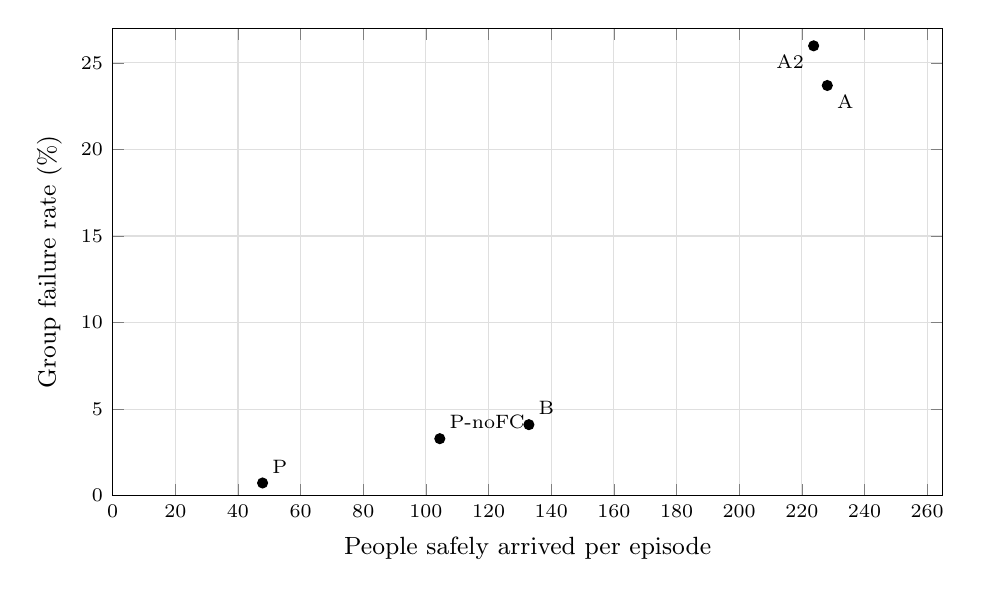
\begin{tikzpicture}
  \begin{axis}[width=\columnwidth, height=0.62\columnwidth,
    xlabel={People safely arrived per episode}, ylabel={Group failure rate (\%)},
    xmin=0, xmax=265, ymin=0, ymax=27, grid=major, grid style={gray!25},
    tick label style={font=\scriptsize}, label style={font=\small}]
    \addplot[only marks, mark=*, mark size=1.8pt] coordinates {
      (228.108,23.692) [A]
      (223.750,25.983) [A2]
      (132.867,4.100) [B]
      (47.858,0.731) [P]
      (104.425,3.290) [P-noFC]
    };
    \node[anchor=north west,font=\scriptsize] at (axis cs:228.108,23.692) {A};
    \node[anchor=north east,font=\scriptsize] at (axis cs:223.750,25.983) {A2};
    \node[anchor=south west,font=\scriptsize] at (axis cs:132.867,4.100) {B};
    \node[anchor=south west,font=\scriptsize] at (axis cs:47.858,0.731) {P};
    \node[anchor=south west,font=\scriptsize] at (axis cs:104.425,3.290) {P-noFC};
  \end{axis}
\end{tikzpicture}

\caption{The trade-off behind the Bar~1 failure (primary regimes). P has the lowest failure rate and
delivers the fewest people of any dispatching system. P-noHyst coincides with P and is omitted; HOLD sits
at the origin.}
\label{fig:tradeoff}
\end{figure}

\paragraph{Q1: no outcome effect (Bar~1 fails).} The certified gate lowered the group failure rate from
\nRateA{} (A) to \nRateP{} (P); E1 $=\nEOneDiff$, 95\,\% CI [\nEOneLo, \nEOneHi]. It did so by
dispatching \nGroupsP{} groups per episode against \nGroupsA{} for A, and it delivered \nSafeP{} people
per episode against \nSafeAtwo{} for A2, so $R=\nR$, far below the 0.95 guard (Table~\ref{tab:systems},
Figure~\ref{fig:tradeoff}). Under the pre-registered rule we make \textbf{no claim that the gate improves
evacuation outcomes}: not better outcomes, not fewer failed trips at equal throughput. Failure rates are
reported only next to $R$.

\paragraph{Secondary contrasts (reported, no bar).} Against B, P's failure rate was lower by
\nPvBDiff{} (CI [\nPvBLo, \nPvBHi]), but B delivered \nSafeB{} people per episode against P's \nSafeP.
P-noFC, which lets through undecided candidates with a high point estimate, dispatched twice as many
groups as P (\nGroupsPnoFC{} vs.\ \nGroupsP) and delivered \nSafePnoFC{} people at a failure rate of
\nFailPnoFC. P-noHyst was identical to P in every episode: P migrated only \nMigrationsP{} times in the
primary regimes, so hysteresis never bound and the ablation is uninformative. For executed P
dispatches, the median absolute difference between the arrival step the rollout predicted in the true
future and the live arrival step was \nArrErrP.

\begin{figure}[t]
\centering
% Generated by scripts/paper_figures.py from frozen files. Do not edit by hand.
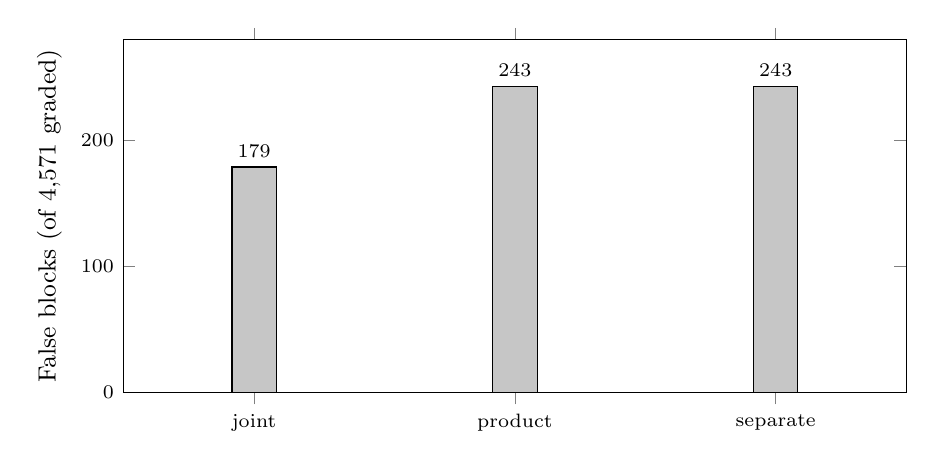
\begin{tikzpicture}
  \begin{axis}[ybar, width=0.95\columnwidth, height=0.5\columnwidth, bar width=16pt,
    symbolic x coords={joint,product,separate}, xtick=data, ymin=0, ymax=280,
    ylabel={False blocks (of \nQtwoGraded{} graded)}, nodes near coords,
    nodes near coords style={font=\scriptsize}, tick label style={font=\scriptsize},
    label style={font=\small}, enlarge x limits=0.25]
    \addplot[fill=gray!45] coordinates {(joint,179) (product,243) (separate,243)};
  \end{axis}
\end{tikzpicture}

\caption{Q2: false blocks among \nQtwoGraded{} graded candidates (\nQtwoCandidates{} sampled, \nQtwoBorderline{}
borderline excluded). No rule made a false accept.}
\label{fig:q2}
\end{figure}

\paragraph{Q2: joint coupling helps at the decision level (Bar~2 passes).} The joint certifier made
\nFBJoint{} errors against \nFBProduct{} for the product of marginals and \nFBSeparate{} for separate
checks; all errors were false blocks, with \nFAJoint, \nFAProduct{} and \nFASeparate{} false accepts
respectively (Figure~\ref{fig:q2}). The joint rule was right on \nMcNJointOnly{} candidates where the
product rule was wrong, and the reverse happened on \nMcNOtherOnly{} ($p=\nMcNp$; \nMcNSepJointOnly{}
vs.\ \nMcNSepOtherOnly{} against separate checks). The false-block reduction against the product of
marginals was \nFBReduction, short of a 30\,\% secondary target.

\paragraph{Q3: keyed common futures did not reduce variance (Bar~3 fails).} The median variance ratio
was \nVarRatio{} over \nQthreeStates{} states, far from the 2$\times$ bar. Keyed futures remain useful for
order invariance and replay, but we claim no variance-reduction effect.

\paragraph{Q4: no false accepts in the sampled states (Bar~4 passes).} \nQfourFA{} of
\nQfourStates{} states contained a false accept (Clopper--Pearson 95\,\% upper bound \nQfourUpper).

\paragraph{Supporting checks.} Replay: \nReplayMatched{} of \nReplayN{} certified decisions from
\nReplaySeeds{} episodes were regenerated bit-for-bit from their stored inputs (a fast test
parameter set, $\epsd=0.30$). Oscillation: in a synthetic study (\nFlipSeeds{} seeds $\times$
\nFlipSteps{} steps, success probabilities following random walks with random collapses, not the
simulator), \nFlipMigrations{} migrations in \nFlipSeedsWithMig{} seeds produced \nFlipReturns{} returns to
a shelter already left and never more than \nFlipMaxMig{} migrations per group. Latency (Q5, laptop,
$n=256$): certify-only p50 \nLatCertPfifty\,ms, p95 \nLatCertPninetyfive\,ms; end-to-end p50
\nLatEtePfifty\,s, p95 \nLatEtePninetyfive\,s. Both targets were missed; the single-board computer and
energy were not measured.

% =====================================================================================================
\section{Discussion: Why a Certified Gate Did Not Help}

The two halves of the result are consistent. Bar~4 says that what the gate certifies has, in the sampled
states, an oracle success probability at or near the threshold or above it; Bar~1 says that holding \emph{every} dispatch to that standard costs
most of the throughput. The rest of this section is interpretation, not pre-registered analysis.

\paragraph{The guarantee is per dispatch; the objective is per person.} E1 is conditional on being
dispatched. A gate that holds people in a flooding zone scores well on E1 while the people it does not
move carry the risk; HOLD dispatches no one and so never fails a trip. A gate deployed for its per-decision
guarantee needs a system-level objective---people safely delivered, time at risk---as its acceptance
criterion, which is why the guard $R$ was in the protocol.

\paragraph{Fail-closed plus multiplicity is conservative by construction.} With $\delta$ split over
$L\cdot A_{\max}$ comparisons and undecided candidates blocked, a candidate needs a true success
probability well above $1-\epsd$ to be certified within 1{,}024 futures; in the Bernoulli check, even with up to 2{,}048 futures, a
candidate at $p=\nCovPNinetySix$ was accepted only \nCovAccNinetySix{} of the time. The P-noFC numbers
are consistent with fail-closed blocking being one large part of the throughput loss, but P-noFC was a
secondary system, not a tested hypothesis.

\paragraph{The joint indicator is the part that travelled.} Evaluating path, shelter and capacity in the
same future rejected fewer feasible dispatches than treating them independently, at no observed safety
cost. Hazards that close roads and degrade shelters share drivers, so marginals misstate the joint
event; this matters for any sample-based safety check over coupled resources, independently of whether
the check is used as a hard gate.

\paragraph{What would have to change.} A gate that should improve outcomes would need its thresholds
chosen against a system-level objective, a different response to UNDECIDED than ``block'' (for example,
escalation to the operator with the evidence), or a cheaper certifier that can afford more futures. Each
of these is a new hypothesis that needs its own pre-registered evaluation; we did not re-run the
evaluation with other parameters.

% =====================================================================================================
\section{Limitations}

Hazards, closures, walk-ins and travel noise are simulated; only the road network is real, and it is a
small extract (\nZones{} zones, \nShelters{} shelters). Futures are generated with the simulator's own
dynamics (from observations, not its latent state), so the model class is right by construction; with a
real forecast the certificate is only as
good as the forecast's calibration (the certifier includes a calibration monitor, unused here). The
evaluated systems run without an operator, while the console requires one. Results come from one
parameter set ($\epsd=0.05$, $\delta=0.01$, up to 1{,}024 futures). The pre-registration was internal, not
public. Latency targets were missed on a laptop, and no field or bench hardware data exist. The
claim-support evaluation behind T2 used construction-labelled pairs written with LLM assistance after an
earlier evaluation had failed; they are not human gold labels.

% =====================================================================================================
\section{Ethics Statement}

No human subjects or personal data were involved; the road data are open data. The guideline corpus is
public; the LLM verifier received only synthetic claims and public guideline text, under a
zero-data-retention setting. The main risk of this line of work is misplaced trust: a ``certified''
label can make a dispatch look safer than the world model behind it warrants, and a fail-closed gate can
\emph{delay} evacuation, shifting risk onto people who are not moved. We therefore report the outcome
failure prominently, show failure rates only next to people delivered, keep a human operator in the
loop in the console, and refuse and log overrides to uncertified actions---a design choice that
itself needs scrutiny by emergency managers before any deployment, since operators may know things the
model does not. Nothing here has been used in a real emergency.

% =====================================================================================================
\section{Conclusion}

We built a fail-closed gate that certifies arrival-time feasibility of each evacuation dispatch over
keyed futures, commits it atomically with a replayable certificate, and re-certifies groups on the road.
Under a pre-registered protocol the gate made no false accept in \nQfourStates{} oracle-checked states and the joint arrival-time indicator was less
wasteful than marginal rules, but the gate delivered \nRpct{} of the people a lookahead planner delivered,
so it does not improve evacuation outcomes as configured. For deployable decision support we read this
as a caution: per-decision safety guarantees should be evaluated, and tuned, against what the system is
for.

% AUTHORS: anonymised; add acknowledgements and the artifact statement only in the camera-ready version,
% after the confidentiality rules are lifted.

\bibliography{refs}

% =====================================================================================================
\appendix
\section{Per-Regime Results}

\begin{table}[h]
\centering\small
\setlength{\tabcolsep}{3pt}
% Generated by scripts/paper_figures.py from frozen files. Do not edit by hand.
\begin{tabular}{@{}llrrrr@{}}
\toprule
System & Regime & Groups & Safe arr./ep. & Fail. rate & Migr.\\
\midrule
HOLD & medium & 0 & 0.0 & -- & 0\\
HOLD & high & 0 & 0.0 & -- & 0\\
HOLD & stress & 0 & 0.0 & -- & 0\\
\addlinespace[2pt]
A & medium & 1{,}045 & 252.6 & 18.0\,\% & 0\\
A & high & 946 & 203.6 & 29.4\,\% & 0\\
A & stress & 944 & 213.7 & 26.1\,\% & 0\\
\addlinespace[2pt]
A2 & medium & 1{,}031 & 252.0 & 18.5\,\% & 0\\
A2 & high & 960 & 195.5 & 33.5\,\% & 0\\
A2 & stress & 962 & 208.2 & 29.3\,\% & 0\\
\addlinespace[2pt]
B & medium & 620 & 167.3 & 4.8\,\% & 0\\
B & high & 362 & 98.4 & 3.4\,\% & 0\\
B & stress & 504 & 138.6 & 3.6\,\% & 0\\
\addlinespace[2pt]
P & medium & 231 & 52.5 & 1.1\,\% & 2\\
P & high & 168 & 43.2 & 0.4\,\% & 0\\
P & stress & 259 & 68.3 & 0.6\,\% & 0\\
\addlinespace[2pt]
P-noFC & medium & 516 & 134.4 & 4.1\,\% & 0\\
P-noFC & high & 275 & 74.5 & 2.5\,\% & 1\\
P-noFC & stress & 428 & 117.6 & 1.6\,\% & 0\\
\addlinespace[2pt]
P-noHyst & medium & 231 & 52.5 & 1.1\,\% & 2\\
P-noHyst & high & 168 & 43.2 & 0.4\,\% & 0\\
P-noHyst & stress & 259 & 68.3 & 0.6\,\% & 0\\
\bottomrule
\end{tabular}

\caption{All systems and regimes, 60 episodes each. Groups: dispatched groups in total; Safe arr./ep.:
mean people safely arrived per episode; Fail. rate: mean per-episode group failure rate; Migr.: migrations
in total. The stress regime is secondary and was not used for any bar.}
\label{tab:regimes}
\end{table}

\section{Reproducibility}
Every number in this paper is generated from frozen result files by one script, which also writes the
tables and figures and a trace from each number to its file and field. Evaluation episodes are seeded and
keyed; the analysis script reproduced its output byte-identically on re-run, and an independent machine
reproduced a subset of baseline episodes (identical except wall time). The mean P episode took
\nPEpisodeSeconds\,s of wall time in the budget run.

\end{document}
